
\chapter{Framework Automated Tuning \label{chap:05-Framework_parameter_tuning}}

% First paragraph has no indentation.

\noindent The models and algorithms from Chapter~\ref{chap:04-Framework-design-and-implementation}
constitute the basis for the radio-coverage framework used throughout
this thesis. Until here, the framework has been studied in the context
of optimization-problem solving for radio networks. In this chapter,
the focus is shifted towards radio-network planning activities, and
how the framework can aid the network-planning engineer in his or
her everyday tasks. The objective is to facilitate refined network
planning, the complexity of which is generally beyond the scope of
any manual approach.

A central part of a radio-planning tool is its radio-propagation model.
Generally speaking, the signal-propagation predictions will be as
accurate as the input data used for their estimation. Moreover, acquiring
and constantly upgrading the necessary data to support the decision
making in this context is an expensive and challenging task. In practical
situations, an emitted signal propagates by interacting with the surrounding
environment. Consequently, the ability of a propagation model to adapt
to the environment where it is used improves the accuracy of the calculated
signal-propagation predictions.

In this context, this chapter presents two automated-tuning capabilities
for PRATO. The first one involves the parameter tuning of the empirical
radio-propagation model using a snapshot of field measurements. The
second one involves the optimization of clutter losses over different
regions of the country, therefore adapting the loss factors to the
local conditions of each region. The results of the experimental simulations,
performed over three regions of a real LTE network deployed by Telekom
Slovenije, d.d., show the suitability of the presented methods to
improve the accuracy of the calculated radio-propagation predictions.

To the best of the author's knowledge, there is no reference in the
literature of an optimization-based approach to automatically adapt
the signal losses due to clutter.

The rest of this chapter is organized as follows. Section~\ref{sec:05-Motivation}
describes the benefits of the presented approach from the radio-planning
point of view. After giving an overview of relevant publications in
Section~\ref{sec:05-Related_work}, the parameter-tuning problem
and two solution approaches are presented in Section~\ref{sec:05-Parameter_tuning_radio-propagation_model},
including the experimental simulations and their results. Section~\ref{sec:05-Clutter_optimization}
concentrates on the description of the optimization problem involving
the regional adaptation of signal losses due to clutter, including
an extensive analysis of the performed simulations on real LTE networks.


\section{Motivation \label{sec:05-Motivation}}

With the advent of LTE as part of the 4G in cellular technology, mobile
operators are facing the challenges of deploying a new network. LTE
follows the well established UMTS/HSPA combo, targeting higher peak
data rates, higher spectral efficiency and lower latency~\cite{Song_Evolved_cellular_network_planning_and_optimization_for_UMTS_and_LTE:2010}. 

The deployment of a new radio network is always a challenge for mobile
operators, who constantly struggle to find the optimal investment
in order to provide a competitive network in terms of coverage and
QoS. Indeed, coverage planning remains a key problem that all operators
have to deal with.

Although different mathematical models have been proposed for radio-propagation
modeling, none of them excels in a network-wide scenario~\cite{Shabbir_Comparison_of_radio_propagation_models:2011}.
Empirical propagation models usually give good results with a limited
computational effort. However, for improved accuracy, the model parameters
have to conform to a specific environment within the network, mainly
because of the inaccuracies in input data and the environmental changes
in the region, e.g., foliage of trees or snow. Consequently, a combination
of different parameters is generally needed in order to reliably calculate
radio-propagation predictions of large networks that cover different
environments.

To address the aforementioned issues, the parameters of an empirical
propagation model are adapted based on a set of field measurements.
A subset of parameters is analytically tuned by computing their values
per cell, in order to increase the accuracy of the calculated predictions.
Also, the full set of parameters is optimized by applying a metaheuristic
approach. Moreover, by applying the same optimization algorithm, the
signal losses due to clutter are automatically adjusted in a regional
basis.

As a simulation framework to evaluate the presented problems, PRATO,
the parallel radio-prediction tool presented in Chapter~\ref{chap:04-Framework-design-and-implementation},
is used. Therefore, the suitability of the framework for planning
and optimization of LTE networks is also validated. Specifically,
PRATO should be capable of handling a large number of radio-propagation
predictions using a metaheuristic algorithm, and a distributed objective-function
evaluation.


\section{Related work \label{sec:05-Related_work}}

Following an optimization-oriented approach, the authors of~\cite{Aarnaes-Tuning_of_empirical_radio_propagation_models_effect_of_location_accuracy:2004}
studied the effects on location accuracy while performing semi-automated
optimization of the parameters of a radio-propagation model. While
their optimization component improves the accuracy of the radio predictions,
it does so requiring human intervention, hence the term semi-automated
optimization. In terms of the effects of location accuracy, they concluded
that locations with a mean accuracy of 60~m may be used for parameter
tuning. Also, they notice that although the model accuracy improved
after the parameter tuning, it gives inadequate results when used
for predicting radio propagation over distant areas.




\section{Parameter tuning of the radio-propagation model \label{sec:05-Parameter_tuning_radio-propagation_model}}

The effectiveness of the decision-making process during radio-network
planning is tightly coupled with the precision achieved by the propagation
model used. In order to obtain a radio-propagation model that most
accurately reflects the propagation characteristics of the area covered
by each radio cell in the network, the parameters of the mathematical
model are adapted to the target environment. Current state-of-the-art
methods for such parameter tuning depend on existing field-measurement
data~\cite{Aarnaes-Tuning_of_empirical_radio_propagation_models_effect_of_location_accuracy:2004,Yang_A_linear_least_square_method_of_propagation_model_tuning_for_3G_radion_network_planning:2008},
which are collected in advance for the area covered by the target
network. Starting from an a-priori best-known set of parameters, manually
calculated by the radio engineers, this approach adapts the model
parameters so that the deviation of the radio-propagation prediction
to a given set of field measurements is minimized.

To calculate the radio-propagation predictions, the OA part of the
empirical model, previously introduced in Section~\ref{sub:04-Radio_propagation_model},
is used. Recall that the model contains a vector of adaptable parameters,
$\vec{\beta}$. For this reason, this mathematical model is especially
appropriate for tuning, since it can be adapted to a given scenario
and its local conditions by adjusting the values of the vector $\vec{\beta}=(\beta_{0},\beta_{1},\beta_{2},\beta_{3})$,
the elements of which represent:
\begin{description}
\item [{$\beta_{0}$}] the reference loss or offset,
\item [{$\beta_{1}$}] the loss slope due to distance of the receiver from
the transmitter,
\item [{$\beta_{2}$}] the loss slope due to height of the transmitter
antenna, and
\item [{$\beta_{3}$}] the loss slope due to the combined effect of the
distance and height of the antenna.
\end{description}
The parameter tuning is performed per cell to improve the local fitting
of the radio predictions, being its resulting solution a vector $\vec{\beta}_{c}^{*}$
for a target cell $c$, $c\in C$.


\subsection{Field measurements \label{sub:05-Field_measurements}}

In radio networks, a UE constantly performs cell selection/reselection
procedures and handover (see Section~\ref{sub:02-Handover-and-soft-handover}),
in order to keep the best possible connection to the network. Within
this context, the best connection is selected by probing a QoS measure
of the neighboring cells. In LTE networks, the UE measures two parameters
from the reference signal of the network, namely the Reference Signal
Received Power (RSRP\nomenclature[A]{RSRP}{Reference signal received power})
and the Reference Signal Received Quality (RSRQ\nomenclature[A]{RSRQ}{Reference signal received quality}).

For a certain frequency bandwidth, RSRP measures the average received
power over the resource elements that carry cell-specific reference
signals. RSRP is applicable in both idle mode (e.g., waiting for a
call) and connected mode (e.g., during a call). During the procedure
of cell selection/reselection in idle mode, RSRP is used, whereas
RSRQ is only applicable when the UE is in connected mode. 

The radio-propagation prediction involves calculating the network
coverage over a certain region. Hence, in the first place, the focus
is on accurately predicting the best connection a UE would select
in idle mode and the RSRP measurements it uses.

Here, the field measurements representing the RSRP at a given location
were collected using a small truck that was equipped with a spectrum
analyzer, the functionality of which supports LTE signal analysis.
The spectrum analyzer was connected to an external omni antenna mounted
on the roof of the truck, at roughly 2~m above the ground, taking
measurements at a rate of 2~Hz. To accurately establish the measurement-location
points, a Global-Positioning-System (GPS\nomenclature[A]{GPS}{Global positioning system})
unit was used. These GPS-informed locations have been tested to be
compliant with the 60~m limit mentioned in~\cite{Aarnaes-Tuning_of_empirical_radio_propagation_models_effect_of_location_accuracy:2004}.
The measurements cover most of the streets within the target area,
with over 300,000 individual points collected for more than 190 network
cells.

To minimize the error in measured RSRP values, and the impact that
small-scale fading has in larger-scale path loss~\cite{Dortmund-Measurement_based_channel_model_for_large_concert_halls:2010},
all field measurements were post-processed so that a single value,
the median, was calculated for each of the measured locations. This
processing step improves measured-data quality in terms of possible
deviations due to external factors, e.g., vehicle driving speed. The
resulting RSRP was then used to estimate the path-loss prediction
at the corresponding location, the resolution of which matches that
of the DEM and clutter data used.


\subsection{Linear least squares \label{sub:05-Linear_least_squares}}

The analytical approach for tailoring the radio-prediction model is
to correlate the RSRP field measurements with the predicted radio-propagation.
The new parameter set originates from the minimization of an error
criterion. Similar to~\cite{Aarnaes-Tuning_of_empirical_radio_propagation_models_effect_of_location_accuracy:2004,Huang_Online_propagation_model_correction_based_on_PSO_algorithm_in_LTE_SON_system:2012,Yang_A_linear_least_square_method_of_propagation_model_tuning_for_3G_radion_network_planning:2008},
the minimization criterion is the squared-sum difference between the
predicted and the observed RSRP levels, i.e.:

\begin{equation}
E(\vec{\beta_{c}})=\sum_{fm\in FM_{c}}(p_{c}-\mathrm{L}{}_{c}(\mathrm{coord}(fm),\vec{\beta_{c}})-fm)^{2}\;\forall c\in C,\label{eq:05-Least_squares_error}
\end{equation}


\noindent where $E(\vec{\beta_{c}})$ is the observed error (in dB)
for cell $c$ given the parameters $\vec{\beta_{c}}$, $C$ is the
cell set of the target network, $p_{c}$ is the transmit power of
cell $c$, and $\mathrm{L}{}_{c}(\mathrm{coord}(fm),\vec{\beta}_{c})$
represents the path loss of cell $c$ at the same geographical point
of the field measurement $fm$, the set of which is $FM_{c}$\nomenclature[S]{$FM_{c}$}{Set of RSRP field measurements for cell $c \in C$}.
Note that $E(\vec{\beta_{c}})$ is independently calculated for each
$c\in C$.

As a general rule when applying this approach, only the first two
components of the vector $\vec{\beta}$ are adapted, i.e., $\beta_{1}$
and $\beta_{2}$, whereas the values of $\beta_{3}$ and $\beta_{4}$
are kept constant~\cite{Huang_Online_propagation_model_correction_based_on_PSO_algorithm_in_LTE_SON_system:2012,Yang_A_linear_least_square_method_of_propagation_model_tuning_for_3G_radion_network_planning:2008}.
Therefore, the analytical method consists in fitting the following
expression, which is reduced from the path-loss definition presented
in Equation~(\ref{eq:04-Hata_OA}):

\begin{equation}
\Delta\mathrm{L}(x,y,\vec{\beta})=\beta_{1}+\beta_{2}\log(d_{(x,y)}).\label{eq:05-lsq_fiting}
\end{equation}


\noindent The expression in Equation~(\ref{eq:05-lsq_fiting}) does
not take the terrain height into account, which is feasible when the
field measurements are taken at a roughly constant height relative
to the base station~\cite{Aarnaes-Tuning_of_empirical_radio_propagation_models_effect_of_location_accuracy:2004,Dalela-Tuning_of_COST_model_for_radio_wave_propagation_predictions:2012,Huang_Online_propagation_model_correction_based_on_PSO_algorithm_in_LTE_SON_system:2012,Yang_A_linear_least_square_method_of_propagation_model_tuning_for_3G_radion_network_planning:2008}.
However, when these heights fluctuate within the coverage area of
a cell, the other two parameters, i.e., $\beta_{3}$ and $\beta_{4}$,
have an effect on the adaptation of the signal-propagation model,
as it will be shown in the following sections.


\subsection{Optimization objective}

The objective of the parameter-optimization problem consists in adjusting
the values of all four components of the vector $\vec{\beta}$, instead
of only two as in the previous section, according to a set of field
measurements of a given cell. Similar to the linear-least-squares
approach, each network cell is independently optimized, so that its
radio-propagation prediction minimizes the mean-squared error against
the field measurements, as defined in Equation~(\ref{eq:05-mean_squared_error}).

\begin{equation}
f_{\mathrm{param}}^{*}(\vec{\beta_{c}})=\min\sum_{fm\in FM_{c}}\frac{(p_{c}-\mathrm{L}{}_{c}(\mathrm{coord}(fm),\vec{\beta_{c}})-fm)^{2}}{\vert FM_{c}\vert}\;\forall c\in C,\label{eq:05-mean_squared_error}
\end{equation}


\noindent where $f_{\mathrm{param}}^{*}(\vec{\beta_{c}})$\nomenclature[S]{$f_{\mathrm{param}}^{*}$}{Objective function of the parameter-tuning problem }
is the optimization objective to be minimized for cell $c$, $FM_{c}$
is the set of all field measurements of cell $c$, the cardinality
of which is $\vert FM_{c}\vert$, and the other parameters are as
denoted previously for Equation~(\ref{eq:05-lsq_fiting}). Note that
$f_{\mathrm{param}}^{*}(\vec{\beta_{c}})$ is independently calculated
for each $c\in C$.


\subsection{Differential ant-stigmergy algorithm}

The chosen optimization algorithm for the parameter-optimization problem
is the DASA (see Section~\ref{sub:02-DASA}). The mapping between
this problem and the DASA is as defined in Equation~(\ref{eq:DASA-parameter_problem_mapping}).

\begin{equation}
X_{a}=\left\{ x_{1},x_{2},x_{3},x_{4}\right\} ,\label{eq:DASA-parameter_problem_mapping}
\end{equation}


\noindent where $X_{a}$ is the solution vector of ant $a$ during
the minimization process, and $x_{j}$, $1\le j\le4$, represents
the $j$-th component of vector $\vec{\beta}$ for the signal-propagation
model of a given cell. At the end of every iteration, and after all
the ants have created solutions, they are evaluated to establish if
any of them is better than the best solution found so far.

There are several reasons for choosing the DASA as the optimization
algorithm in the context of this problem. First, the benefits of metaheuristic
algorithms for solving optimization problems, particularly in the
context of radio networks, was demonstrated by several authors in
general~\cite{Benedicic_Balancing_downlink_uplink_soft_handover_areas_in_UMTS_networks:2012,Garcia-Lozano_Metaheuristic_procedure_to_optimize_transmission_delays_in_DVB-T_single_frequency_networks:2011,Huang_Online_propagation_model_correction_based_on_PSO_algorithm_in_LTE_SON_system:2012,Malla_Energy_efficient_resource_allocation_in_OFDMA_networks_using_ant_colony_optimization:2012},
and in this thesis in particular (see Chapters~\ref{chap:02-Optimization_of_radio_networks},
\ref{chap:06-Experimental-evaluation-the-service-coverage-problem}
and~\ref{chap:07-Experimental-evaluation-the-SHO-alignment-problem}).
Second, in~\cite{korosec2010_DASA}, the authors validated the suitability
of the algorithm for solving numerical-optimization problems.

After some trial-optimization runs, the six parameters that control
the way the DASA explores the search space were set to the following
values:
\begin{itemize}
\item $m=80$, the number of ants;
\item $b=10,$ the discrete base;
\item $\rho=0.2$, the pheromone dispersion factor;
\item $s_{+}=0.01$, the global scale-increasing factor;
\item $s_{-}=0.01$, the global scale-decreasing factor; and 
\item $\epsilon=10^{-5}$, the maximum parameter precision.
\end{itemize}
The trial runs consisted in doubling $m$ from 5 to 640, and verifying
the convergence profile and best solution found. The values of the
other parameters were left unchanged.


\subsection{Simulations \label{sub:05-Simulations}}

The first simulation round consisted in building the matrices of the
observed-error values, $E(\vec{\beta_{c}})$, for each cell $c$ in
the target network. The linear systems of equations were then individually
solved by applying the linear least-squares method, which involves
the evaluation of one radio-coverage prediction per cell. Each solved
system holds a unique solution for a cell $c$, $c\in C$, denoted
by the vector $\vec{\beta_{c}^{*}}$.

The second simulation round involved multiple iterations of several
steps. The process began with a cell set of a mobile network and a
set of field measurements, which were gathered before-hand through
drive tests. Together with the mobile-network configuration and layout,
they provide the input data for the optimization process itself. An
iteration begins when the DASA generates a solution vector for each
of the ants in the colony. The following step involves the parallel
evaluation of the solution vector carried by an ant, i.e., one radio-propagation
prediction per worker process of PRATO. The objective-function value
is calculated as defined in Equation~(\ref{eq:05-mean_squared_error}),
and sent back to the DASA for it to generate the next set of solutions.
The optimization process involves multiple iterations, which are repeated
until some stopping criteria are met. Then, the best solution found
represents the optimized values of the parameters of the radio-propagation
model of the target cell. Figure~\ref{fig:05-PRATO_architecture_optimization}
depicts the described system elements and their relationships for
the parameter-optimization problem.

Compared with the analytical approach, that requires the solution
of a linear system of equations, a large number of evaluations is
needed for the DASA to converge to a solution. Therefore, it is essential
to exploit the parallel nature of PRATO in order to evaluate the radio-coverage
prediction of multiple cells within a network. Otherwise, such approach
would not be feasible, since the time required to reach a reasonable
solution would be excessive.

The stopping criteria for the optimization runs limited the maximum
number of objective-function evaluations, the value of which was set
to 50 for all the test networks.

\begin{figure}
\centering

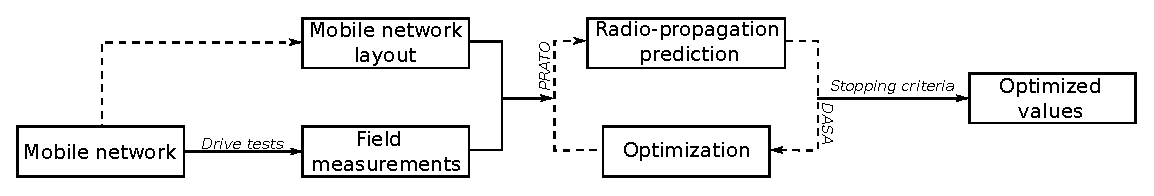
\includegraphics[width=0.9\textwidth]{05-framework_parameter_tuning/img/process_diagram}

\caption{\textit{\emph{The automatic-tuning system, including its elements
and their relationships. \label{fig:05-PRATO_architecture_optimization}}}}
\end{figure}


\bigskip{}



\subsubsection*{Test networks}

The test networks, Net$_{8}$, Net$_{9}$, and Net$_{10}$, are subsets
of a real LTE network deployed in Slovenia by Telekom Slovenije, d.d.
The path-loss predictions are calculated using PRATO, with a DEM and
clutter map of 25~m$^{2}$ resolution, and a receiver height of 2~m
above ground level. A transmission radius defines the coverage-prediction
area around each network transmitter, thus limiting the path-loss
prediction to a distance where it is feasible for a UE to connect
to a cell, with a RSRP greater or equal to -124~dBm~\cite{Neuland_Influence_of_Different_Factors_on_X_Map_Estimation_in_LTE:2011}.
At the same time, the selected transmission radius provides enough
overlap among neighboring cells to calculate the network coverage
over the whole region. Table~\ref{tab:05-Test_network_properties}
provides detailed information about the test networks used, including
the number of network cells, the area surface, and the covering proportion
of the collected field measurements in terms of the total area of
each test network.

\begin{table}
\centering

\caption{Parameters of the test networks Net$_{8}$, Net$_{9}$ and Net$_{10}$
that were used for the experimental simulations during the automated
tuning of the radio-propagation model.\label{tab:05-Test_network_properties}}


{\footnotesize{}}%
\begin{tabular}{cccccc}
\cline{2-6} 
 & {\footnotesize{Number of cells }} & {\footnotesize{Transmission radius {[}km{]}}} & {\footnotesize{Area type}} & {\footnotesize{Area {[}km$^{2}${]}}} & {\footnotesize{Drive-tests area {[}\%{]}}}\tabularnewline
\hline 
{\footnotesize{Net$_{8}$ }} & {\footnotesize{12}} & {\footnotesize{16.00}} & {\footnotesize{Rural}} & {\footnotesize{82.90}} & {\footnotesize{4.75}}\tabularnewline
{\footnotesize{Net$_{9}$ }} & {\footnotesize{156 }} & {\footnotesize{8.00}} & {\footnotesize{Urban}} & {\footnotesize{468.30}} & {\footnotesize{22.31}}\tabularnewline
{\footnotesize{Net$_{10}$ }} & {\footnotesize{26 }} & {\footnotesize{16.00}} & {\footnotesize{Hilly}} & {\footnotesize{133.47}} & {\footnotesize{10.92}}\tabularnewline
\hline 
\end{tabular}
\end{table}


Net$_{8}$ represents a network deployed over a dominant agricultural
area with almost flat terrain, some forests and water streams. Net$_{9}$
is deployed over a densely populated urban area, containing high buildings,
parks and avenues. The last one, Net$_{10}$, represents a network
deployed over hilly terrain, including some smaller villages and vast
forests.

Since the terrain profiles are most relevant for Net$_{8}$ and Net$_{10}$,
they are shown in Figures~\ref{fig:05-Terrain_profile_for_Net8}
and~\ref{fig:05-Terrain_profile_for_Net10}, respectively. Note that
the terrain shown in Figure~\ref{fig:05-Terrain_profile_for_Net8}
is mostly flat, since the agricultural area prevails in Net$_{8}$.
In contrast, the terrain for Net$_{10}$ is dominated by hills, which
are mostly covered by forests, including some small villages in the
valleys (see Figure~\ref{fig:05-Terrain_profile_for_Net10}).

\begin{figure}
\begin{minipage}[t]{0.49\textwidth}%
\centering

\includegraphics[width=1\columnwidth]{\lyxdot \lyxdot /tun_par/doc/img/terrain_MS}

\caption{Terrain profile of the test network Net$_{8}$, dominated by a flat
agricultural area. \label{fig:05-Terrain_profile_for_Net8}}
%
\end{minipage}\hfill{}%
\begin{minipage}[t]{0.49\textwidth}%
\centering

\includegraphics[width=1\columnwidth]{\lyxdot \lyxdot /tun_par/doc/img/terrain_HI}

\caption{Terrain profile of the test network Net$_{10}$, dominated by forested
hills. \label{fig:05-Terrain_profile_for_Net10}}
%
\end{minipage}
\end{figure}


In the following, the manually-calculated, default parameters of the
radio-propagation model correspond to the values provided by the engineers
of the Radio Network department at Telekom Slovenije, d.d.

\bigskip{}


The simulations were carried out on several computing nodes of the
previously presented DEGIMA cluster~\cite{Hamada_Cluster_of_GPUs:2010}
at the NACC of the Nagasaki University in Japan (see Section~\ref{sec:04-Simulations}).
Groups of 4, 12, and 40 nodes were used for executing the simulations
of the different problem instances, i.e., Net$_{8}$, Net$_{9}$ and
Net$_{10}$, respectively.


\subsection{Results \label{sub:05-Least_squares_results}}

The results of calculating the radio-propagation predictions with
different parameter sets are presented in this section. The analysis
to fit the parameters of the radio-propagation model to a set of field
measurements is given with the default parameters, after applying
the linear least-squares method, and after applying the metaheuristic-optimization
method. The mean and standard-deviation values were calculated correlating
the field measurements with the radio-propagation prediction of each
test network.

Bar charts were prepared to show the probability distribution functions
(PDFs\nomenclature[A]{PDF}{Probability distribution function}) of
the difference between the radio-propagation predictions and the field
measurements (see Figures~\ref{fig:05-Error_distribution_for_Net8},
\ref{fig:05-Error_distribution_for_Net9}, and \ref{fig:05-Error_distribution_for_Net10}).
Each bar represents an open interval denoting the proportion of measurement
points that deviate from the prediction in the given number of dB.

Figure~\ref{fig:05-Error_distribution_for_Net8}~(a) depicts the
PDF of the coverage prediction for test network Net$_{8}$ using the
empirically-calculated parameters, Figure~\ref{fig:05-Error_distribution_for_Net8}~(b)
shows the difference distribution for the same test network, but using
the analytically-calculated parameters, and Figure~\ref{fig:05-Error_distribution_for_Net8}~(c)
shows the difference distribution using the DASA-optimized parameters.
Notice how the difference distributions show an improvement when the
analytically-calculated parameters are used, lowering the largest
(outer) deviations, and raising the lowest (inner) ones. Additionally,
the difference is negligible when using the optimized parameters,
thus confirming that it is sufficient to only adapt $\beta_{0}$ and
$\beta_{1}$ in environments where the height difference between the
base station and the receiver (i.e., $\log(H_{\mathrm{A}})$ in Equation~(\ref{eq:04-Hata_OA}))
is roughly constant, e.g., a rural area.

The PDFs test network Net$_{9}$ using the default, fitted and optimized
parameters are shown in Figures~\ref{fig:05-Error_distribution_for_Net9}~(a),
\ref{fig:05-Error_distribution_for_Net9}~(b) and \ref{fig:05-Error_distribution_for_Net9}~(c),
respectively. The fitted parameters represent a significant accuracy
improvement when compared with the default ones. Similar to Net$_{8}$,
the optimized parameters show a negligible improvement when compared
to the fitted ones. This is due to the height difference between the
base-station antenna and the receiver having almost no variations
throughout the area covered by the drive tests.

The difference distributions of the radio-propagation predictions
for test network Net$_{10}$ using the manually-calculated parameters,
the analytically-calculated, and the optimized ones are shown in Figures~\ref{fig:05-Error_distribution_for_Net10}~(a),
\ref{fig:05-Error_distribution_for_Net10}~(b), and \ref{fig:05-Error_distribution_for_Net10}~(c),
respectively. Similar to Net$_{8}$, the improvement appears in the
largest deviations, since their values are lower than when using the
manually-calculated parameters. In this case, we may also observe
the improvement achieved by the DASA-optimized parameters, the optimization
of which included all four components of the vector $\vec{\beta}$,
thus better reflecting the signal propagation over the hilly terrain.

The presented results confirm that the parameter optimization of the
signal-propagation model with respect to field measurements improves
the quality of the calculated radio-propagation predictions. Considering
the default parameter values were manually calculated by the radio
engineers for the whole network, the convenience of the automated
optimization procedure is clear. Indeed, these advantages are a consequence
of a simpler method that delivers radio-predictions of superior quality,
thus accurately representing the physical properties of a given environment.

\begin{figure}
\centering

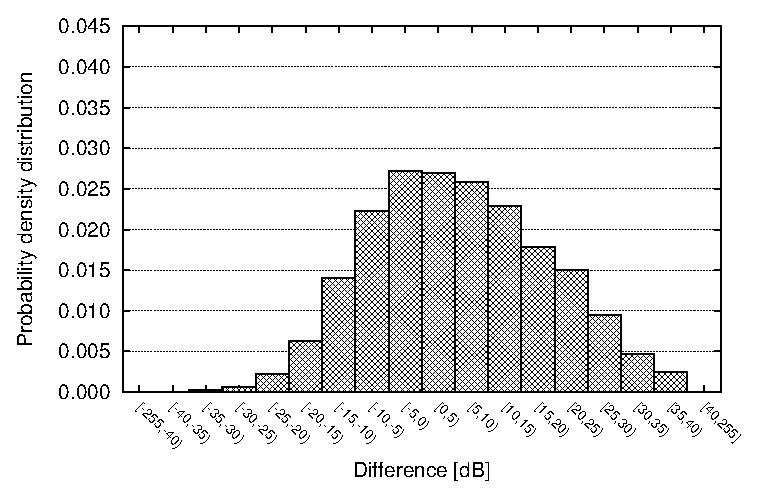
\includegraphics[width=0.63\textwidth]{05-framework_parameter_tuning/img/rural-default_distribution}\\\hspace*{0.3in}(a)\vspace{5mm}

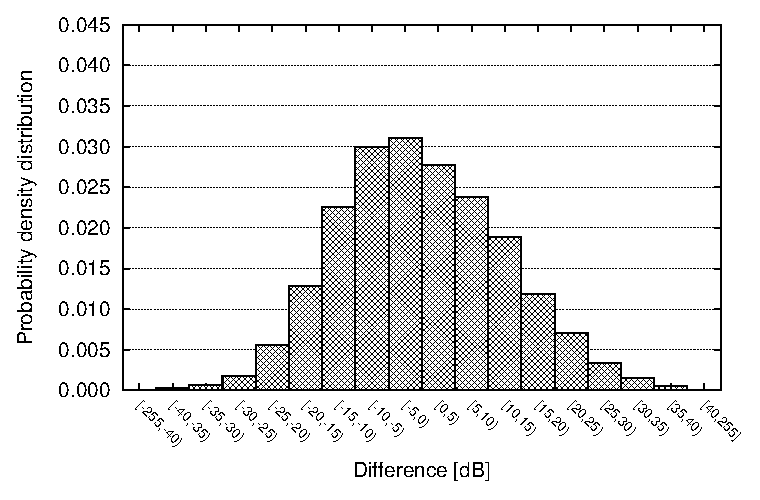
\includegraphics[width=0.63\textwidth]{05-framework_parameter_tuning/img/rural-fitted_distribution}\\\hspace*{0.3in}(b)\vspace{5mm}

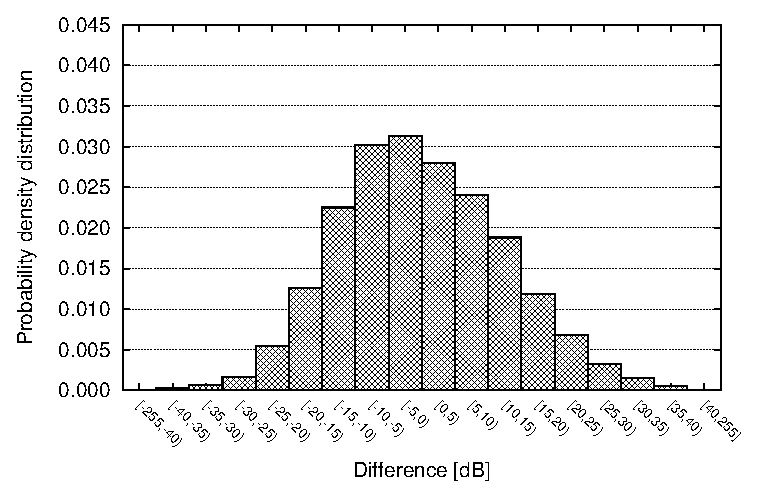
\includegraphics[width=0.63\textwidth]{05-framework_parameter_tuning/img/rural-optim_distribution}\\\hspace*{0.3in}(c)\vspace{5mm}\caption{Probability-density distribution of radio predictions against the
field measurements of network Net$_{8}$ over a rural area using the:
(a) empirically-calculated parameters, (b) analytically-calculated
parameters, and (c) optimized parameters.\label{fig:05-Error_distribution_for_Net8}}
\end{figure}


\begin{figure}
\centering

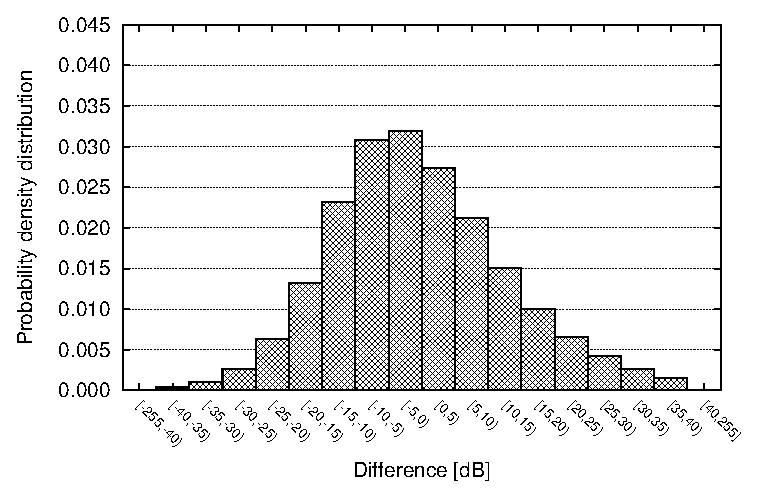
\includegraphics[width=0.63\textwidth]{05-framework_parameter_tuning/img/urban-params_default}\\\hspace*{0.3in}(a)\vspace{5mm}

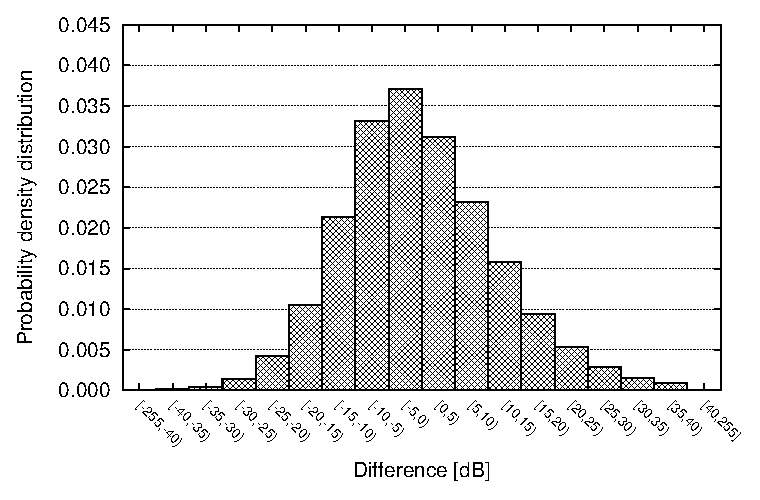
\includegraphics[width=0.63\textwidth]{05-framework_parameter_tuning/img/urban-params_fitted}\\\hspace*{0.3in}(b)\vspace{5mm}

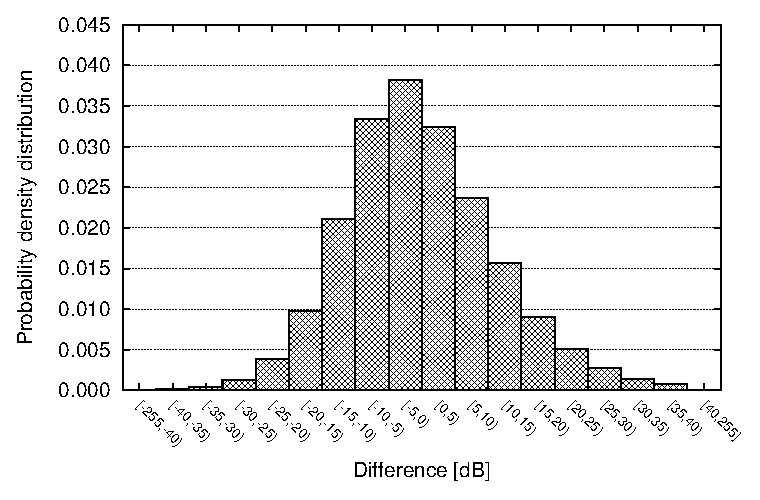
\includegraphics[width=0.63\textwidth]{05-framework_parameter_tuning/img/urban-params_optim}\\\hspace*{0.3in}(c)\vspace{5mm}

\caption{Probability-density distribution of radio predictions against the
field measurements of network Net$_{9}$ over an urban area using
the: (a) empirically-calculated parameters, (b) analytically-calculated
parameters, and (c) optimized parameters.\label{fig:05-Error_distribution_for_Net9}}
\end{figure}


\begin{figure}
\centering

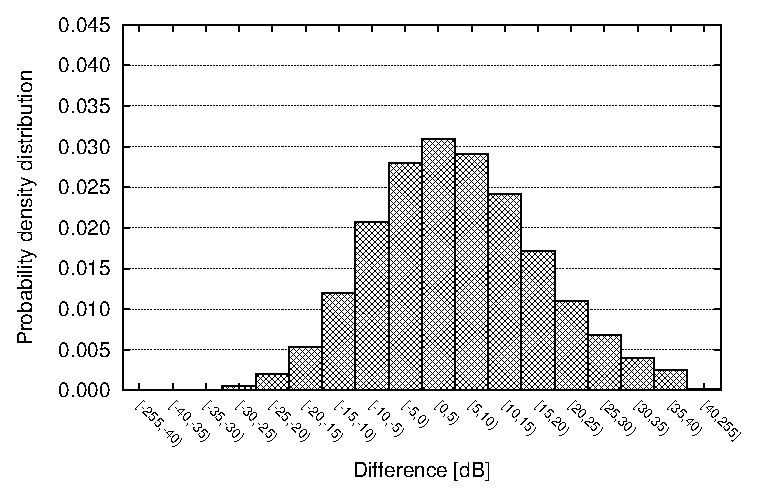
\includegraphics[width=0.63\textwidth]{05-framework_parameter_tuning/img/hilly-default_distribution}\\\hspace*{0.3in}(a)\vspace{5mm}

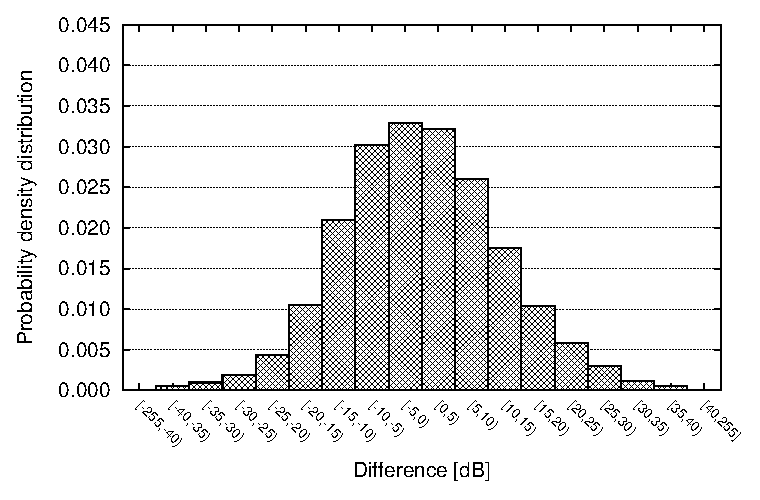
\includegraphics[width=0.63\textwidth]{05-framework_parameter_tuning/img/hilly-fitted_distribution}\\\hspace*{0.3in}(b)\vspace{5mm}

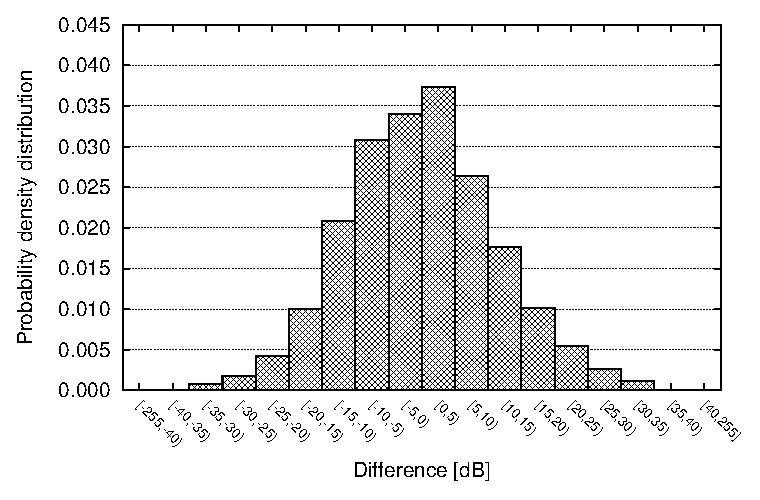
\includegraphics[width=0.63\textwidth]{05-framework_parameter_tuning/img/hilly-optim_distribution}\\\hspace*{0.3in}(c)\vspace{5mm}

\caption{Probability-density distribution of radio predictions against the
field measurements of network Net$_{10}$ over a hilly area using
the: (a) empirically-calculated parameters, (b) analytically-calculated
parameters, and (c) optimized parameters.\label{fig:05-Error_distribution_for_Net10}}
\end{figure}



\subsection{Performance analysis}

{\small{}}
\begin{table}
\centering

\caption{Mean and standard-deviation values of the radio-propagation prediction
against the field measurements. The values, expressed in dB, are given
when using the manual, analytical and DASA approaches for each test
network. \label{tab:05-Solution_analysis}}


{\small{}}%
\begin{tabular}{cccccccccc}
\cline{2-10} 
 & \multicolumn{3}{c}{{\small{Manual}}} & \multicolumn{3}{c}{{\small{Analytical}}} & \multicolumn{3}{c}{{\small{DASA}}}\tabularnewline
\hline 
{\small{Test network}} &  & {\small{Mean}} & {\small{Std. dev.}} &  & {\small{Mean}} & {\small{Std. dev.}} &  & {\small{Mean}} & {\small{Std. dev.}}\tabularnewline
\hline 
{\small{Net$_{8}$}} &  & {\small{5.88496}} & {\small{13.69240}} &  & {\small{0.00001}} & {\small{12.64708}} &  & {\small{0.01974}} & {\small{12.13723}}\tabularnewline
{\small{Net$_{9}$}} &  & {\small{0.07172}} & {\small{13.94477}} &  & {\small{0.00001}} & {\small{12.13115}} &  & {\small{0.01504}} & {\small{11.82010}}\tabularnewline
{\small{Net$_{10}$}} &  & {\small{6.52300}} & {\small{14.35561}} &  & {\small{0.00007}} & {\small{12.30833}} &  & {\small{0.01372}} & {\small{10.59590}}\tabularnewline
\hline 
\end{tabular}
\end{table}
{\small \par}

Table~\ref{tab:05-Solution_analysis} shows the solutions reached
by each of the compared approaches for the three test networks. The
calculated mean and standard-deviation values are depicted in terms
of the difference between the calculated radio-propagation predictions
and the field measurements.

We may observe that the standard deviation improved for all test networks
when using DASA as the optimization approach. Although the value of
the mean measure is higher in this case than when applying the analytical
method, it is consistently lower than 0.05~dB, which is a negligible
difference in the context of radio-propagation predictions. Regarding
the lower standard-deviation measure for test network Net$_{10}$,
the value of which improved by almost 2~dB, it shows a significant
gain in the accuracy of the radio-propagation predictions. This is
especially important on the borders of cell coverage, where a 2~dB
difference in the received-signal strength could mean predicting sufficient
network coverage where there will be none.


\section{Clutter optimization \label{sec:05-Clutter_optimization}}

In order to further improve the accuracy of the radio-prediction calculation
over a given regional environment, the signal losses due to clutter
are optimized in this section.

As it was mentioned before, there are several reasons for the predicted
signal-loss values to be inaccurate. The seasonal changes are among
them, like tree foliage and snow. Also, changes related to urban development,
like demolition or construction of buildings and parks, and different
kinds of forests or agricultural areas, etc. These changes are only
noticeable through regular updates of accurate land-usage data. However,
in the short term, updates are only available in the form of feedback
by means of drive-tests campaigns for field-measurement gathering.

In the following, a metaheuristic algorithm is used to optimize the
clutter losses of a target radio network. This is done over groups
of network cells within different regions of the target network, e.g.,
agricultural, urban or hilly. In terms of coverage planning, a regional
classification of the signal losses due to clutter improves the accuracy
of the radio-coverage prediction.

Similar to the parameter tuning of the mathematical model presented
in Section~\ref{sec:05-Parameter_tuning_radio-propagation_model},
the DASA metaheuristic algorithm is once again the tool of choice
for optimizing the clutter losses.

Recall that in Equation~(\ref{eq:04-Hata_pathloss}), the model includes
an extra term in order to adequately predict signal-loss effects due
to foliage, buildings and other fabricated structures. These loss
factors are based on the land usage, known as clutter data. Here,
eleven different clutter categories are recognized. Table~\ref{tab:05-Clutter_categories}
lists these categories, including their label numbers and descriptions. 

\begin{table}
\centering

\caption{Clutter-category label numbers and descriptions for the signal loss
due to clutter, as reflected by a radio-propagation model. \label{tab:05-Clutter_categories}}


\begin{tabular}{cl}
\hline 
Clutter category & Description\tabularnewline
\hline 
1 & Suburban area \tabularnewline
2 & Urban area\tabularnewline
3 & Dense urban area\tabularnewline
4 & Agricultural area\tabularnewline
5 & Forest area\tabularnewline
6 & Swamp area\tabularnewline
7 & Dry open land area with special vegetation\tabularnewline
8 & Dry open land area without special vegetation\tabularnewline
9 & Water area\tabularnewline
10 & Industrial area\tabularnewline
11  & Park area\tabularnewline
\hline 
\end{tabular}
\end{table}



\subsection{Optimization objective \label{sub:Optimization-objective}}

The optimization objective consists of adjusting the loss values of
the different clutter categories, i.e., $\mathrm{L}{}_{\mathrm{CLUT}}(d_{(x,y)})$
as used in Equation~(\ref{eq:04-Hata_pathloss}), according to a
set of field measurements of a given geographical region. The same
three data sets used in Section~\ref{sub:05-Simulations} were used
for the clutter-optimization problem: the first for Net$_{8}$, the
second for Net$_{9}$, and the third for Net$_{10}$. Each region
was independently optimized, so that the radio-propagation predictions
of each set of cells per test network minimized the total mean-squared
error against the field measurements, based on the previously defined
objective function in Equation~(\ref{eq:05-mean_squared_error}),
i.e.:

\begin{equation}
f_{\mathrm{clut}}^{*}=\min\sum_{c\in C}f_{\mathrm{param}}^{*}(\vec{\beta_{c}^{*}}),\label{eq:05-clutter_problem_objective}
\end{equation}


\nomenclature[S]{$f^{*}_{\mathrm{clut}}$}{Objective function of the clutter-optimization problem}

\noindent where $\vec{\beta_{c}^{*}}$ is the optimized parameter
vector for cell $c$ as calculated previously in Section~\ref{sub:05-Simulations}.

\bigskip{}


In this case, the mapping between the clutter-optimization problem
and the DASA is as follows:

\begin{equation}
X_{a}=\left\{ x_{1},\ldots,x_{i},\ldots,x_{11}\right\} ,\label{eq:DASA-problem_mapping}
\end{equation}


\noindent where $X_{a}$ is the solution vector of ant $a$ during
the minimization process, and $x_{i}$ represents the $i$-th clutter
category within a given region or network.


\subsection{Simulations}

In this case, only one simulation round was performed for the DASA.
The work flow of the optimization process, and the test networks used,
are the same as for the parameter-optimization problem described previously
in Section~\ref{sub:05-Simulations} and Figure~\ref{fig:05-PRATO_architecture_optimization}.

For a clearer characterization of the test networks in terms of the
available field measurements and terrain types, the proportions of
each clutter category with respect to the total area covered by the
drive tests are shown in Table~\ref{tab:05-Proportion_of_clutter_for_test_networks}.

\begin{table}
\centering

\caption{Field-measurement proportions with respect to each clutter category,
the percentages of which are given in terms of the area covered by
the drive tests for each of the test networks. The clutter category
legend is given in Table~\ref{tab:05-Clutter_categories}. \label{tab:05-Proportion_of_clutter_for_test_networks}}


{\small{}}%
\begin{tabular}{crrr}
\hline 
{\small{Clutter category}} & {\small{Net$_{1}$~{[}\%{]}}} & {\small{Net$_{2}$~{[}\%{]}}} & {\small{Net$_{3}$~{[}\%{]}}}\tabularnewline
\hline 
{\small{1}} & {\small{12.77}} & {\small{9.23}} & {\small{8.34}}\tabularnewline
{\small{2}} & {\small{27.57}} & {\small{35.99}} & {\small{31.17}}\tabularnewline
{\small{3}} & {\small{3.10}} & {\small{7.34}} & {\small{4.15}}\tabularnewline
{\small{4}} & {\small{48.24}} & {\small{33.05}} & {\small{41.13}}\tabularnewline
{\small{5}} & {\small{5.19}} & {\small{8.29}} & {\small{8.59}}\tabularnewline
{\small{6}} & {\small{0.00}} & {\small{0.00}} & {\small{0.10}}\tabularnewline
{\small{7}} & {\small{0.00}} & {\small{0.05}} & {\small{0.00}}\tabularnewline
{\small{8}} & {\small{0.39}} & {\small{0.02}} & {\small{0.04}}\tabularnewline
{\small{9}} & {\small{0.21}} & {\small{0.58}} & {\small{3.00}}\tabularnewline
{\small{10}} & {\small{2.53}} & {\small{4.74}} & {\small{3.37}}\tabularnewline
{\small{11 }} & {\small{0.00}} & {\small{0.71}} & {\small{0.11}}\tabularnewline
\hline 
{\small{Drive-test area}} & {\small{100.00}} & {\small{100.00}} & {\small{100.00}}\tabularnewline
\hline 
\end{tabular}
\end{table}


In agreement with previous related research about clutter losses~\cite{Rubinstein-Clutter_losses:1998,Shamsan-Fixed_wireless_service:2011},
and since no clutter generates greater attenuation than 40~dB, we
limited the optimized clutter losses to the interval {[}0,40{]}.

The stopping criteria for the optimization runs was set by limiting
the maximum number of objective-function evaluations. In this sense,
the limits for Net$_{8}$ and Net$_{10}$ were set the 200, whereas
for Net$_{9}$ the value was 500, since this network contains the
largest number of cells. Overall, the framework completed 48,000 objective-function
evaluations, i.e., 576,000 radio-coverage predictions for Net$_{8}$
and 288,000 for Net$_{10}$, whereas for Net$_{9}$, the number of
objective-function evaluations was 120,000, for a total of 15,600,000
radio-coverage predictions.

Regarding the parameters that control the behavior of the DASA, they
were set to the following values after some trial-optimization runs:
\begin{itemize}
\item $m=240$, the number of ants;
\item $b=10,$ the discrete base;
\item $\rho=0.2$, the pheromone dispersion factor;
\item $s_{+}=0.01$, the global scale-increasing factor;
\item $s_{-}=0.01$, the global scale-decreasing factor; and 
\item $\epsilon=10{}^{-2}$, the maximum parameter precision.
\end{itemize}
The trial runs consisted in doubling $m$ from 15 to 480, and verifying
the convergence profile and best solution found. The values of the
other parameters were left unchanged.


\subsection{Results}

\begin{table}
\centering

\caption{Clutter-category losses after the optimization. The default losses
for each clutter category are given along the solutions for each of
the test networks. All values are expressed in dB. \label{tab:05-Clutter_optimization_solutions}}


{\small{}}%
\begin{tabular}{ccccc}
\hline 
{\small{Clutter category}} & {\small{Default}} & {\small{Net$_{8}$}} & {\small{Net$_{9}$}} & {\small{Net$_{10}$}}\tabularnewline
\hline 
{\small{1}} & {\small{13.0}} & {\small{18.43}} & {\small{15.10}} & {\small{14.79}}\tabularnewline
{\small{2}} & {\small{15.0}} & {\small{19.66}} & {\small{16.34}} & {\small{15.94}}\tabularnewline
{\small{3}} & {\small{28.0}} & {\small{16.92}} & {\small{19.83}} & {\small{22.21}}\tabularnewline
{\small{4}} & {\small{12.0}} & {\small{9.50}} & {\small{11.58}} & {\small{11.85}}\tabularnewline
{\small{5}} & {\small{20.0}} & {\small{14.63}} & {\small{13.22}} & {\small{11.79}}\tabularnewline
{\small{6}} & {\small{15.0}} & {\small{-}} & {\small{-}} & {\small{14.57}}\tabularnewline
{\small{7}} & {\small{8.0}} & {\small{-}} & {\small{12.79}} & {\small{-}}\tabularnewline
{\small{8}} & {\small{5.0}} & {\small{3.85}} & {\small{9.78}} & {\small{0.68}}\tabularnewline
{\small{9}} & {\small{1.0}} & {\small{3.99}} & {\small{9.67}} & {\small{7.10}}\tabularnewline
{\small{10}} & {\small{20.0}} & {\small{12.85}} & {\small{16.49}} & {\small{15.62}}\tabularnewline
{\small{11 }} & {\small{8.0}} & {\small{-}} & {\small{19.16}} & {\small{15.01}}\tabularnewline
\hline 
\end{tabular}
\end{table}


The results achieved by the optimization process are shown in Table~\ref{tab:05-Clutter_optimization_solutions}.
The solutions are given for each of the test networks, along with
the manually-calculated (default) loss values. These default values
were provided by the radio experts of the Radio Network department
at Telekom Slovenije, d.d. Hyphens represent clutter categories for
which there were no field measurements available. Consequently, it
was not possible to evaluate the objective-function for them.

The optimized loss for the first clutter category, 1, representing
suburban area, is above the default one for all test networks, indicating
a building density above the average. For category 2, representing
urban area, the optimized values are again above the default ones,
clearly showing underestimation of the manual approach. Despite this,
the relation with the suburban clutter losses is correctly kept, i.e.,
the signal losses are higher in each test network. In contrast with
category 1, the optimized values of category 3, representing dense
urban area, are lower than the default one. This indicates that dense
urban areas in these regions have a lower density than the average
case. Representing agricultural area, category 4 gets a value very
close to the default one for Net$_{9}$ and Net$_{10}$, whereas for
Net$_{8}$ the value is lower, indicating that this type of land is
mostly open there. As for category 5, representing forests, the results
correspond with the type of forest dominating each of the test networks.
Namely, Net$_{8}$ and Net$_{9}$ are dominated by dense forests presenting
leave foliage, whereas in Net$_{10}$ the forests are mostly coniferous
and more sparse. Keeping the default loss values for categories 6
and 7, category 8, representing open land without special vegetation,
the optimized values of which vary significantly, mostly influenced
by the low proportion of field measurements over this type of land
in each region. As for category 9, representing water, the results
of which indicate creeks and rivers in all regions are surrounded
by forests (Net$_{8}$), buildings (Net$_{9}$), and hills and forests
(Net$_{10}$), since none of the regions lays by the sea. As for the
industrial area, denoted by clutter category 10, lower loss values
than the manually-calculated default appear. This indicates the presence
of sparse industrial buildings in Net$_{8}$, and a higher density
of mostly commercial buildings for Net$_{9}$ and Net$_{10}$. Finally,
the last clutter category 11 could not be calculated for Net$_{8}$
since there are not parks there, whereas the values for Net$_{9}$
and Net$_{10}$ agree with the region type, i.e., urban and hilly,
respectively.

It is important to note that the relation among different clutter
categories within a region is correctly kept. For example, we may
observe that the clutter loss for urban area (category 2) is higher
than those for the suburban area (category 1), as well as for category
4 (agricultural area). Hence, the results reflect physically feasible
losses, despite the higher deviation from the default losses shown
by category 3, and the lower deviation for category 4, again with
respect to the default losses. Such relations hold for different categories
in all test networks, strongly suggesting the correctness of the applied
optimization approach and the evaluation methodology used.

Based on these observations and after summarizing the extensive experimentation,
the results obtained indicate that the use of a metaheuristic algorithm
to perform automatic optimization of clutter losses is clearly applicable
for radio-propagation predictions in LTE networks. Most notably, the
proposed approach is capable of reflecting the physical phenomena
appearing in real-world conditions within geographically-different
network instances that contain a large number of cells.

\bigskip{}


\begin{figure}
\centering

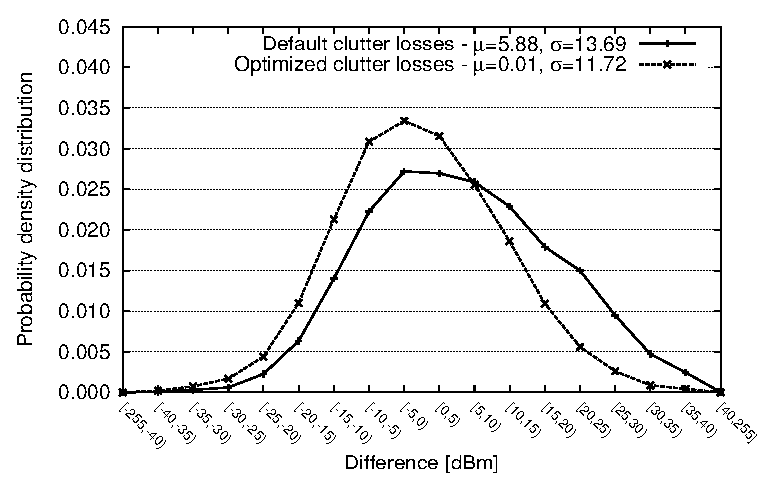
\includegraphics[width=0.62\textwidth]{05-framework_parameter_tuning/img/rural-diff_distribution}

\caption{Probability density function of the difference between the radio-propagation
prediction and the field measurements for network Net$_{8}$ over
a rural area.\label{fig:05-Clutter_error_distribution_for_Net8}}


\vspace{-0.5cm}
\end{figure}


\begin{figure}
\centering

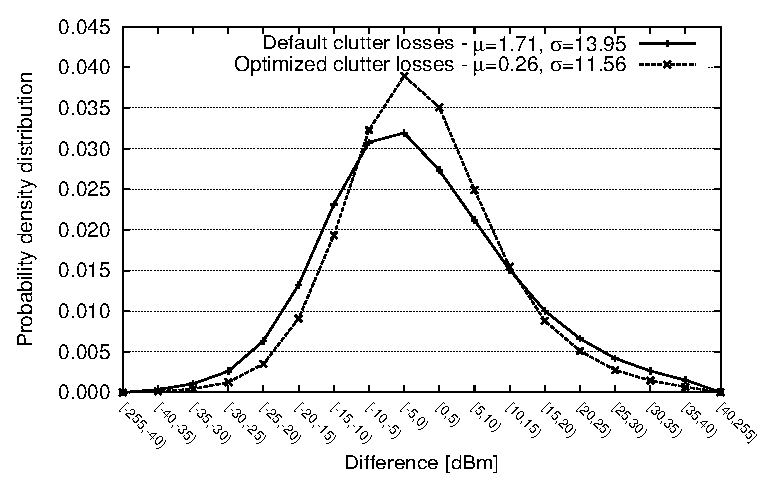
\includegraphics[width=0.62\textwidth]{05-framework_parameter_tuning/img/urban-diff_distribution}

\caption{Probability density function of the difference between the radio-propagation
prediction and the field measurements for network Net$_{9}$ over
an urban area.\label{fig:05-Clutter_error_distribution_for_Net9}}


\vspace{-0.5cm}
\end{figure}


\begin{figure}
\centering

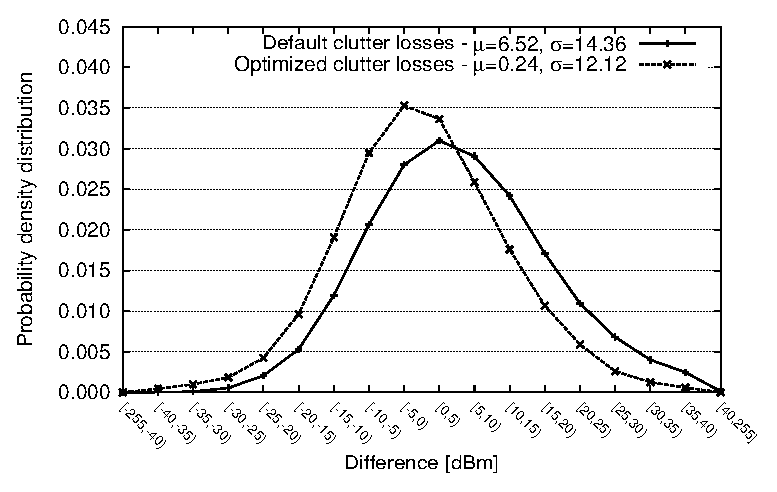
\includegraphics[width=0.62\textwidth]{05-framework_parameter_tuning/img/hilly-diff_distribution}

\caption{Probability density function of the difference between the radio-propagation
prediction and the field measurements for network Net$_{10}$ over
a hilly area.\label{fig:05-Clutter_error_distribution_for_Net10}}
\end{figure}


Similar to Section~\ref{sub:05-Least_squares_results}, charts were
prepared to show the PDFs of the difference between the signal-propagation
predictions and the field measurements, the values of which are expressed
in dBm. Figure~\ref{fig:05-Clutter_error_distribution_for_Net8}
depicts the distribution of the difference between the coverage prediction
for test network Net$_{8}$ using the default clutter losses, and
using the optimized clutter losses (see Table~\ref{tab:05-Clutter_optimization_solutions},
column Net$_{8}$). Notice how the distribution shows an improvement
when the optimized clutter losses are used, lowering the largest (outer)
differences, and raising the lowest (inner) ones. The mean of the
PDF was reduced from 5.88 when using the default clutter losses, to
0.01 with the optimized losses; whereas the standard deviation was
reduced from 13.69 to 11.72, respectively.

The difference distributions of the radio-propagation predictions
for test network Net$_{9}$ using default and optimized clutter losses
are shown in Figure~\ref{fig:05-Clutter_error_distribution_for_Net9}.
Again, an improvement can be noticed in its shape, clearly showing
the favorable effects of the optimization process. In this case, the
mean value dropped from 1.71 to 0.26, whereas the standard deviation
was reduced from 13.95 to 11.56.

For the last test network, Net$_{10}$, the difference distributions
are depicted in Figure~\ref{fig:05-Clutter_error_distribution_for_Net10}.
Similar to Net$_{8}$, the variations appear in the largest difference
values, since they are lower than when using the default clutter losses.
Regarding the improvement of the mean of the PDFs with the default
and optimized clutter losses, they were 6.52, and 0.23, respectively;
whereas the standard deviation was reduced from 14.36 to 12.12, respectively.

The presented results confirm that the optimization of clutter losses
with respect to field measurements improves the accuracy of the calculated
radio-propagation predictions. Considering the default clutter losses
were manually calculated by the radio engineers for the whole network,
there is a clear advantage for the presented automatic optimization
procedure. It follows that the accurate representation of the physical
properties in a given environment produces more precise radio-propagation
predictions.


\subsection{Performance analysis}

\begin{table}
\centering

\caption{Statistical analysis of the solutions for the clutter-optimization
problem. All values are expressed in dB. The corresponding box plots
are depicted in Figure~\ref{fig:05-Statistical_analysis_boxplots}.
\label{tab:05-Statistical_analysis_of_solutions}}


{\scriptsize{}}%
\begin{tabular}{>{\centering}p{0.2cm}cccc>{\centering}p{0.75cm}cccc>{\centering}p{0.75cm}cccc>{\centering}p{0.75cm}}
\cline{3-16} 
 &  &  & \multicolumn{2}{c}{{\scriptsize{Net$_{8}$}}} &  &  &  & \multicolumn{2}{c}{{\scriptsize{Net$_{9}$}}} &  &  &  & \multicolumn{2}{c}{{\scriptsize{Net$_{10}$}}} & \tabularnewline
\hline 
{\scriptsize{Cat.}} &  & {\scriptsize{Min}} & {\scriptsize{Max}} & {\scriptsize{Avg}} & {\scriptsize{St.dev.}} &  & {\scriptsize{Min}} & {\scriptsize{Max}} & {\scriptsize{Avg}} & {\scriptsize{St.dev.}} &  & {\scriptsize{Min}} & {\scriptsize{Max}} & {\scriptsize{Avg}} & {\scriptsize{St.dev.}}\tabularnewline
\hline 
{\scriptsize{1}} &  & {\scriptsize{18.37}} & {\scriptsize{18.49}} & {\scriptsize{18.43}} & {\scriptsize{0.04}} &  & {\scriptsize{15.83}} & {\scriptsize{16.27}} & {\scriptsize{16.11}} & {\scriptsize{0.14}} &  & {\scriptsize{14.42}} & {\scriptsize{15.26}} & {\scriptsize{14.79}} & {\scriptsize{0.24}}\tabularnewline
\cline{1-6} \cline{8-11} \cline{13-16} 
{\scriptsize{2}} &  & {\scriptsize{19.61}} & {\scriptsize{19.71}} & {\scriptsize{19.66}} & {\scriptsize{0.02}} &  & {\scriptsize{17.05}} & {\scriptsize{17.15}} & {\scriptsize{17.10}} & {\scriptsize{0.02}} &  & {\scriptsize{15.66}} & {\scriptsize{16.09}} & {\scriptsize{15.94}} & {\scriptsize{0.13}}\tabularnewline
\cline{1-6} \cline{8-11} \cline{13-16} 
{\scriptsize{3}} &  & {\scriptsize{16.89}} & {\scriptsize{16.97}} & {\scriptsize{16.92}} & {\scriptsize{0.12}} &  & {\scriptsize{19.80}} & {\scriptsize{21.22}} & {\scriptsize{20.28}} & {\scriptsize{0.28}} &  & {\scriptsize{21.78}} & {\scriptsize{22.57}} & {\scriptsize{22.21}} & {\scriptsize{0.26}}\tabularnewline
\cline{1-6} \cline{8-11} \cline{13-16} 
{\scriptsize{4}} &  & {\scriptsize{9.47}} & {\scriptsize{9.52}} & {\scriptsize{9.50}} & {\scriptsize{0.01}} &  & {\scriptsize{11.55}} & {\scriptsize{11.72}} & {\scriptsize{11.64}} & {\scriptsize{0.06}} &  & {\scriptsize{11.64}} & {\scriptsize{12.05}} & {\scriptsize{11.85}} & {\scriptsize{0.11}}\tabularnewline
\cline{1-6} \cline{8-11} \cline{13-16} 
{\scriptsize{5}} &  & {\scriptsize{14.57}} & {\scriptsize{14.69}} & {\scriptsize{14.63}} & {\scriptsize{0.04}} &  & {\scriptsize{10.20}} & {\scriptsize{10.85}} & {\scriptsize{10.49}} & {\scriptsize{0.21}} &  & {\scriptsize{11.50}} & {\scriptsize{12.17}} & {\scriptsize{11.79}} & {\scriptsize{0.22}}\tabularnewline
\cline{1-6} \cline{8-11} \cline{13-16} 
{\scriptsize{6}} &  & {\scriptsize{-}} & {\scriptsize{-}} & {\scriptsize{-}} & {\scriptsize{-}} &  & {\scriptsize{-}} & {\scriptsize{-}} & {\scriptsize{-}} & {\scriptsize{-}} &  & {\scriptsize{11.68}} & {\scriptsize{16.99}} & {\scriptsize{14.57}} & {\scriptsize{1.67}}\tabularnewline
\cline{1-6} \cline{8-11} \cline{13-16} 
{\scriptsize{7}} &  & {\scriptsize{-}} & {\scriptsize{-}} & {\scriptsize{-}} & {\scriptsize{-}} &  & {\scriptsize{9.51}} & {\scriptsize{15.06}} & {\scriptsize{12.76}} & {\scriptsize{1.81}} &  & {\scriptsize{-}} & {\scriptsize{-}} & {\scriptsize{-}} & {\scriptsize{-}}\tabularnewline
\cline{1-6} \cline{8-11} \cline{13-16} 
{\scriptsize{8}} &  & {\scriptsize{3.37}} & {\scriptsize{4.79}} & {\scriptsize{3.85}} & {\scriptsize{0.27}} &  & {\scriptsize{2.15}} & {\scriptsize{8.55}} & {\scriptsize{4.75}} & {\scriptsize{1.98}} &  & {\scriptsize{0.00}} & {\scriptsize{2.28}} & {\scriptsize{0.68}} & {\scriptsize{1.90}}\tabularnewline
\cline{1-6} \cline{8-11} \cline{13-16} 
{\scriptsize{9}} &  & {\scriptsize{3.81}} & {\scriptsize{4.18}} & {\scriptsize{3.99}} & {\scriptsize{0.09}} &  & {\scriptsize{9.02}} & {\scriptsize{14.17}} & {\scriptsize{11.77}} & {\scriptsize{1.25}} &  & {\scriptsize{6.45}} & {\scriptsize{7.43}} & {\scriptsize{7.10}} & {\scriptsize{0.34}}\tabularnewline
\cline{1-6} \cline{8-11} \cline{13-16} 
{\scriptsize{10}} &  & {\scriptsize{12.76}} & {\scriptsize{12.94}} & {\scriptsize{12.85}} & {\scriptsize{0.07}} &  & {\scriptsize{16.20}} & {\scriptsize{17.36}} & {\scriptsize{16.69}} & {\scriptsize{0.50}} &  & {\scriptsize{15.33}} & {\scriptsize{16.02}} & {\scriptsize{15.62}} & {\scriptsize{0.31}}\tabularnewline
\cline{1-6} \cline{8-11} \cline{13-16} 
{\scriptsize{11}} &  & {\scriptsize{-}} & {\scriptsize{-}} & {\scriptsize{-}} & {\scriptsize{-}} &  & {\scriptsize{17.89}} & {\scriptsize{20.26}} & {\scriptsize{19.05}} & {\scriptsize{0.81}} &  & {\scriptsize{11.97}} & {\scriptsize{17.51}} & {\scriptsize{15.01}} & {\scriptsize{1.43}}\tabularnewline
\hline 
\end{tabular}
\end{table}


\begin{figure}
\centering

\includegraphics[width=0.65\textwidth]{05-framework_parameter_tuning/img/boxplot-rural}\\\hspace*{0.2in}(a)

\includegraphics[width=0.65\textwidth]{05-framework_parameter_tuning/img/boxplot-urban}\\\hspace*{0.2in}(b)

\includegraphics[width=0.65\textwidth]{05-framework_parameter_tuning/img/boxplot-hilly}\\\hspace*{0.2in}(c)

\caption{Box plots representing the statistical-analysis values of Table~\ref{tab:05-Statistical_analysis_of_solutions},
for the solutions of the clutter-optimization process of each test
network: (a)~Net$_{8}$, (b)~Net$_{9}$, and (c)~Net$_{10}$.\label{fig:05-Statistical_analysis_boxplots}}
\end{figure}


\bigskip{}


Because of the stochastic nature of the DASA, the results of 30 independent
runs were collected in order to have enough data for them to be statistically
relevant. In other words, the robustness of the solutions that were
presented in the previous section is analyzed here.

To this end, Table~\ref{tab:05-Statistical_analysis_of_solutions}
shows the solutions reached by the DASA for each of three test networks.
The calculated signal losses are depicted with the minimum, maximum
and average values for every clutter category, along with their standard
deviations. Again, hyphens represent clutter categories for which
there were no field measurements available, and thus they could not
be optimized. In order to easily visualize the data shown in Table~\ref{tab:05-Statistical_analysis_of_solutions},
box plots based on the same values are depicted in Figure~\ref{fig:05-Statistical_analysis_boxplots}. 

It can be observed that the standard deviation is low for almost all
optimized categories, indicating a consistent convergence of the optimization
algorithm. However, we notice some exceptions, e.g., categories 7
and 8 in Net$_{9}$, and 6, 8 and 11 in Net$_{10}$. There is a particularly
low proportion of field measurements for the enumerated clutter categories
(see Table\ \ref{tab:05-Proportion_of_clutter_for_test_networks}).
Indeed, higher standard deviation values consistently appear for clutter
categories with fewer field measurements. Therefore, and based on
the obtained results, the standard deviation of the optimized clutter
losses provides a quantity indicator of the field measurements required
by the optimization process, i.e., a higher standard deviation denotes
more field measurements are needed over these areas in order to improve
the optimization results the target clutter category.


\section{Summary}

This chapter illustrated the suitability of PRATO as a network-planning
tool by tackling two coverage-planning problems, which were tested
over the newly deployed LTE network in Slovenia. The first one involved
the parameter tuning of the empirical radio-propagation model using
a snapshot of field measurements. The second one considered the optimization
of the clutter losses over different sub-networks of the country,
therefore automatically adapting them to the local conditions of the
geographical region of each network.

The combination of the aforementioned techniques with PRATO provides
an environment-adaptable framework for radio-network planning. This
delivers a tool with considerably improved solution accuracy of the
analyzed instances, especially if compared to traditional, i.e., manual
or semi-automated, coverage-planning methods.

Additionally, the simulation results indicate that PRATO is applicable
for planning and optimization of real-world radio networks, since
it is capable of simulating a large number of coverage configurations
in a feasible amount of time. In particular, several of the presented
instances show a large computational-time complexity, which is beyond
reach for a serial implementation of an automated approach. Moreover,
the parallelization capabilities provided by the framework create
new problem-solving possibilities, together with the automation of
tasks that have been traditionally performed manually by the network
engineers. Furthermore, even computational-intensive tasks such as
objective-function evaluations for stochastic optimization are feasible
if PRATO is used.

To the best of the author's knowledge, an automatic-optimization method
for the clutter losses of a geographical area has not yet been presented
in the related literature.
